
\documentclass{article} % For LaTeX2e
\usepackage{iclr2026_conference,times}

% Optional math commands from https://github.com/goodfeli/dlbook_notation.
\input{math_commands.tex}

% \usepackage{hyperref}
\definecolor{cvprblue}{rgb}{0.21,0.49,0.74}
\usepackage[breaklinks,colorlinks,citecolor=cvprblue]{hyperref}
\usepackage{url}

% New packages and commands
\usepackage[ruled]{algorithm2e} % For algorithms
\renewcommand{\algorithmcfname}{ALGORITHM}
\SetAlFnt{\small}
\SetAlCapFnt{\small}
\SetAlCapNameFnt{\small}
\SetAlCapHSkip{0pt}

\newcommand{\mycommentstyle}[1]{\color[HTML]{0671b9}{\small #1}}
\SetKwComment{Comment}{\mycommentstyle{// }}{}
\definecolor{mycommentcolor}{HTML}{0671b9}

\newcommand{\todo}[1]{\textcolor{purple}{[TODO] \emph{#1}}}
\newcommand{\anyi}[1]{\textcolor{red}{[Anyi] #1}}

\usepackage{bm}
\usepackage{booktabs} % For formal tables
\usepackage{graphicx}
\usepackage{makecell}
\usepackage{subcaption}

\usepackage[capitalize]{cleveref}
\crefname{section}{Sec.}{Secs.}
\Crefname{section}{Section}{Sections}
\Crefname{table}{Table}{Tables}
\crefname{table}{Tab.}{Tabs.}
\Crefname{algorithm}{Algorithm}{Algorithms}
\crefname{algorithm}{Alg.}{Algs.}

% Add a period to the end of an abbreviation unless there's one
% already, then \xspace.
\makeatletter
\DeclareRobustCommand\onedot{\futurelet\@let@token\@onedot}
\def\@onedot{\ifx\@let@token.\else.\null\fi\xspace}

\def\eg{\emph{e.g}\onedot} \def\Eg{\emph{E.g}\onedot}
\def\ie{\emph{i.e}\onedot} \def\Ie{\emph{I.e}\onedot}
\def\cf{\emph{cf}\onedot} \def\Cf{\emph{Cf}\onedot}
\def\etc{\emph{etc}\onedot} \def\vs{\emph{vs}\onedot}
\def\wrt{w.r.t\onedot} \def\dof{d.o.f\onedot}
\def\iid{i.i.d\onedot} \def\wolog{w.l.o.g\onedot}
\def\etal{\emph{et al}\onedot}
\makeatother

\newcommand{\sref}[1]{\S\ref{#1}}
\newcommand{\sssection}[1]{\noindent\textbf{#1}}


\title{Taming Flow-based I2V Models for\\Creative Video Editing}

% Authors must not appear in the submitted version. They should be hidden
% as long as the \iclrfinalcopy macro remains commented out below.
% Non-anonymous submissions will be rejected without review.

\author{
% Antiquus S.~Hippocampus, Natalia Cerebro \& Amelie P. Amygdale \thanks{ Use footnote for providing further information
% about author (webpage, alternative address)---\emph{not} for acknowledging
% funding agencies.  Funding acknowledgements go at the end of the paper.} \\
% Department of Computer Science\\
% Cranberry-Lemon University\\
% Pittsburgh, PA 15213, USA \\
% \texttt{\{hippo,brain,jen\}@cs.cranberry-lemon.edu}
% \\
% \And
% Ji Q. Ren \& Yevgeny LeNet \\
% Department of Computational Neuroscience \\
% University of the Witwatersrand \\
% Joburg, South Africa \\
% \texttt{\{robot,net\}@wits.ac.za} \\
% \AND
Xianghao Kong$^1$, Hansheng Chen$^2$, Yuwei Guo$^3$, Lvmin Zhang$^2$,\\ ~\textbf{Gordon Wetzstein$^2$, Maneesh Agrawala$^2$, Anyi Rao$^1$} \\
$^1$~HKUST, $^2$~Stanford University, $^3$~CUHK \\
% Address \\
% \texttt{email}
}

% The \author macro works with any number of authors. There are two commands
% used to separate the names and addresses of multiple authors: \And and \AND.
%
% Using \And between authors leaves it to \LaTeX{} to determine where to break
% the lines. Using \AND forces a linebreak at that point. So, if \LaTeX{}
% puts 3 of 4 authors names on the first line, and the last on the second
% line, try using \AND instead of \And before the third author name.

\newcommand{\fix}{\marginpar{FIX}}
\newcommand{\new}{\marginpar{NEW}}

\iclrfinalcopy % Uncomment for camera-ready version, but NOT for submission.
\begin{document}

\maketitle

\begin{figure}[h!]
  \vspace{-3pt}
  \centering
  \includegraphics[width=\linewidth]{figs/teaser.pdf}
  \caption{Illustration of IF-V2V, a lightweight plug-and-play method for creative video editing (\sref{sec:intro}). It effectively combines the capability of black-box image editing approaches and flow-matching-based I2V models without inversion and optimization, achieving various creative editing tasks with high visual quality.}
  \label{fig:teaser}
\end{figure}

\begin{abstract}
Although image editing techniques have advanced significantly, video editing, which aims to manipulate videos according to user intent, remains an emerging challenge.
% Video editing, which aims to manipulate input videos towards the user's intention, is still in its infancy compared to well-developed image editing approaches. 
Most existing image-conditioned video editing methods either require inversion with model-specific design or need extensive optimization, limiting their capability of leveraging up-to-date image-to-video (I2V) models to transfer the editing capability of image editing models to the video domain. 
% To this end, we propose IF-V2V, an inversion-free image-conditioned video editing method that can be applied to any flow-matching-based I2V models without optimization. 
To this end, we propose IF-V2V, an \underline{I}nversion-\underline{F}ree method that can adapt off-the-shelf flow-matching-based I2V models for video editing without significant computational overhead.
To circumvent inversion, we devise Vector Field Rectification with Sample Deviation to incorporate information from the source video into the denoising process by introducing a deviation term into the denoising vector field. To further ensure consistency with the source video in a model-agnostic way, we introduce Structure-and-Motion-Preserving Initialization to generate motion-aware temporally correlated noise with structural information embedded. We also present a Deviation Caching mechanism to minimize the additional computational cost for denoising vector rectification without significantly impacting editing quality. Evaluations demonstrate that our method achieves superior editing quality and consistency over existing approaches, offering a lightweight plug-and-play solution to realize visual creativity.
\end{abstract}

\section{Introduction}

Recently, agent systems based on Large Language Models (LLMs) have attracted significant research interest. With the rapid development of AI technologies, LLM-based agent systems dynamically handle complex tasks in various interactive environments, alleviating human burdens. Agent systems are increasingly applied across diverse fields~\citep{liu2025advances}, including clinical treatment~\citep{wang2025surveyllmbasedagentsmedicine}, scientific simulations~\citep{park2023generativeagentsinteractivesimulacra}, and software engineering~\citep{wang2025openhandsopenplatformai}.

Despite the considerable attention agent systems have received, their security remains an urgent area for improvement~\citep{wang2025comprehensivesurvey,yu2025asurveytrustagent}. One security topic previously discussed in cybersecurity yet still crucial in agent systems, is \textbf{access control (AC)}. To minimize the loss caused by privilege escalation or unexpected behavior, systems require optimal permission allocation strategies that are adapted to the generative behavior patterns of LLM-based agents. Traditional AC models, built on static rules and binary allow/deny logic~\citep{ferraiolo2009rolebasedaccesscontrols,8594462}. Early research proposed formal methods based on Information Flow Control (IFC)~\citep{myers1997decentralized} to allocate permissions, ensuring secure interactions among system entities. Subsequent advances extended these mechanisms to incorporate contextual factors such as user role, location, and time
~\citep{covington2001context}. Unfortunately, traditional IFC mechanisms face severe limitations in handling dynamic, implicit semantics or complex interactive behaviors, which renders agent access control vulnerable. Our vision paper underscores the importance of access control in agent systems, and argues that strategies for permission allocation must \textbf{move beyond the traditional focus on securing static data, to instead emphasize the governance of dynamic information flow.} Therefore, we envision \textbf{Agent Access Control (AAC)} as a novel framework which redefines access control not as an external security gate, but as an intrinsic cognitive capability of the agent itself. The core of AAC is to view information disclosure as a process of judging appropriateness based on reasoning and context, rather than relying only on fixed rules.

To realize this vision, our AAC framework is built upon two integrated modules, executed by a dedicated reasoning engine: (1) Multi-dimensional Contextual Evaluation, which analyzes the holistic context of an interaction, and (2) Adaptive Response Formulation, which crafts nuanced, appropriate information outputs. In the following content, we begin by detailing the framework, then explore the critical role of its core reasoning engine for effective access control. Finally, the future implications and challenges of this new paradigm will be presented to pave the way for agents that are not only capable, but trustworthy.


\section{Related Work}
\label{sec:related}

\sssection{Image-to-video Generation.} Visual content generation and editing have witnessed significant advancements thanks to the emergence of diffusion models~\citep{ddpm, ddim, ldm}. Recently, DiT~\citep{dit} has become the mainstream architecture of the denoising model with promising generation quality, surpassing U-Net~\citep{unet} with its powerful scaling capability~\citep{kaplan2020scalinglawsneurallanguage} and potential for multimodal interaction~\citep{sd3}. Flow Matching~\citep{flowmatching, rectifiedflow} introduces an improved generative model paradigm that interpolates data and noise linearly in the forward diffusion process, bringing better theoretical properties and conceptual simplicity. Building upon these works, a number of I2V models~\citep{wan, easyanimate, hunyuanvideo, cogvideox, opensora2, vchitect2} have emerged with full 3D attention~\citep{attention2017} instead of decoupled spatiotemporal attention~\citep{guo2024animatediff}, significantly enhancing generation quality and consistency.

% Image-conditioned video editing methods leverage the temporal prior of I2V models to propagate the edited keyframe along the temporal dimension while preserving structure and motion consistency with the source video. Videoshop~\citep{videoshop} introduces noise extrapolation to enhance the inversion process. DreamMotion~\citep{dreammotion} utilizes score distillation sampling (SDS)~\citep{pooledreamfusion} to optimize the source video latents towards the condition image, during which space-time self-similarities constraints are applied to better match the source video. I2VEdit~\citep{i2vedit} first trains a sample-specific motion LoRA~\citep{lora} and then performs attention matching between the EDM~\citep{edm} inversion and denoising process. AnyV2V~\citep{kuanyv2v} performs DDIM~\citep{ddim} inversion and exploits an attention injection paradigm to ensure consistency with the source video. VideoRepainter~\citep{videorepainter} repurposes an I2V model for editing by fine-tuning it with a symmetric condition mechanism to avoid mask ambiguity caused by downsampling. VACE~\citep{vace} provides an all-in-one solution for video editing by introducing a ControlNet-style~\citep{controlnet} Context Adapter structure, which requires extensive training. These approaches include either model-specific designs or costly optimization, limiting their ability to keep up with the rapid advancement of I2V models.

\sssection{Training-free Visual Editing.} Training-free visual editing modifies the source image or video according to designated conditions (e.g., text, image, and mask) at test time, using off-the-shelf pretrained models. Existing works can be broadly categorized into two categories: inversion-based and optimization-based methods. Inversion-based methods~\citep{videoshop, dni, wave, yatim2025dynvfxaugmentingrealvideos} adopt the inversion of the diffusion process to map the input back to Gaussian noise, and then perform denoising under given conditions. However, not only is the inversion process time-consuming, but it also inevitably induces error. To overcome the inherent inaccuracy of inversion and ensure consistency with the input, various attention injection strategies~\citep{wave, yatim2025dynvfxaugmentingrealvideos} are utilized to further incorporate source information. Despite their effectiveness, these strategies are model-specific, reducing their universality to different model structures. Optimization-based methods~\citep{dreammotion, ren2025fdsfrequencyawaredenoisingscore, unityindiversity} use SDS~\citep{pooledreamfusion} to directly optimize the input latents towards the desired direction. Nevertheless, the optimization operation introduces considerable computational cost, limiting its availability to common creators. With the prevalence of flow-based models~\citep{flowmatching, rectifiedflow}, there have also been methods~\citep{avrahami2025stableflowvitallayers, dalva2024fluxspacedisentangledsemanticediting, xu2025unveilinversioninvarianceflow} that leverage the properties of the flow matching process to achieve more precise and consistent visual editing. However, few solutions are both lightweight and universal without model-specific design in the video domain, limiting creators to swiftly leverage the most up-to-date I2V base models for video editing within user-friendly resources, such as a single GPU.
% to take the temporal dimension into account.

There have also been works exploring inversion-free image editing. For instance, InfEdit~\citep{infedit} theoretically depends on the diffusion process, limiting its application to state-of-the-art flow-based models. It also needs attention manipulation, further limiting its universality. FlowEdit~\citep{kulikov2024floweditinversionfreetextbasedediting} leverages flow properties to construct a transport from the source to the target distribution, which is derived from the Euler Discrete Solver~\citep{sd3}. In contrast, our method constructs two parallel ODEs to model the editing process, which does not depend on a specific ODE solver and enables control over editing strength. Our method also introduces SMPI to further enhance video-level spatiotemporal consistency and a flexible caching strategy.

\section{Method}
%
Next, we formulate the target task and describe the training data generation and representation learning. 
An overview of the proposed generation process is shown in \cref{fig:overview}.

\subsection{Task formulation}
%
The target task is instance-level image retrieval.
Given a query image, the goal is to retrieve all positive images from a database (db), \ie those that depict the same object instance as the query.
Images depicting different object instances, even if they belong to the same semantic category, are negatives and should not be retrieved.
This is an open-world task, testing on unseen objects from a variety of domains which may be seen or unseen during training.

We consider the efficient retrieval variant using global descriptors.  
Formally, an image $x$ is mapped to a $d$-dimensional global descriptor $\mathbf{z} = f_\theta(x) \in \mathbb{R}^d$.  
Retrieval is performed via nearest neighbor search in Euclidean space, ranking database descriptors based on their cosine similarity to the query.  
The encoder, parameterized by $\theta$, is optimized during training.
We focus on fine-tuning foundational models~\citep{zhai2023sigmoid} that already perform well by pretraining.  

\begin{figure*}[t]
% \vspace{5pt}
\centering
\includegraphics[width=.95\linewidth]{fig/overview.pdf}
% \vspace{-5pt}
\caption{Overview of instance-level training data generation.
A domain name or description is the only input, which is used to prompt an LLM to provide a list of object category names. 
Then, we generate examples of those categories using a GDM, remove the background, and synthesize lighting and background multiple times per generated example to create a diverse set of positive images for each instance.
} 
\label{fig:overview}
\end{figure*}

\subsection{Instance-level training data generation}
%
We propose a pipeline that requires only the name, or a textual description, of a target domain as input, and automatically generates an image training set with instance-level labels.
The process consists of four stages:
(i) \textit{Objects categories generation} by prompting an LLM to provide a list of %useful 
object category names;
(ii) \textit{Object instance generation} by prompting a GDM to generate object instances from each category;
(iii) \textit{Background generation} by synthesizing diverse backgrounds per instance;
(iv) \textit{Viewpoint variations} by augmenting the generated images with geometric transformations.
Each stage of the process is detailed below.

\paragraph{Object categories generation}
%
Object categories (\eg \textit{table}, \textit{chair}, \textit{clock}) are needed to prompt the GDM for image generation. 
We automatically obtain a list of object categories by prompting an LLM with minimal information about the domain of interest. 
In the general case in which we do not target a specific domain, the prompt we use is 
``\emph{Provide a raw list of names of everyday objects.}''
For specific domains, such as artwork, landmark, or product, we enrich the prompt with relevant information and hint with a few examples of object categories. 
Full details of the designed prompts are provided in the supplementary material. 
This approach yields a rich and diverse list of $C$ object categories.
Examples of category names generated for the general case are \textit{sofa}, \textit{desk}, while for the specific domains are \textit{bust}, \textit{castle}, and \textit{polaroid film}, for artwork, landmark, and product, respectively.

\paragraph{Object instance generation}
%
We prompt a GDM, in particular Stable Diffusion Turbo~\citep{sauer2025adversarial}, with an object category to generate $K$ images per category.
We assume that generating images with different random seeds produces variations that are distinct and recognizable as separate instances within the same category. 
Therefore, following an instance-level class definition, each of the $M$ generated images, where $M = C K$, is treated as a separate class in our training set.
To facilitate the follow-up step of background generation, we target a simple or uniform background. To achieve this, we add ``\emph{in a clean background}" to the prompt after the object category as in, ``\textit{a table in a clean background}." 
%
Examples in \cref{fig:sdimages} show that, even though the background removal process may fail in both cases, it is less likely to happen with the extended prompt, while the original prompt provides outputs with richer background.


\begin{figure*}[t]
\begin{center}    
% \vspace{5pt}
\footnotesize
\newcommand{\figclean}[2]{\includegraphics[width=42pt,height=42pt]{fig/sd/#1/clean/#2.png}&\includegraphics[width=42pt,height=42pt]{fig/sd/#1/clean/#2_fg.png}}
\newcommand{\figunclean}[2]{\includegraphics[width=42pt,height=42pt]{fig/sd/#1/unclean/#2.png}&\includegraphics[width=42pt,height=42pt]{fig/sd/#1/unclean/#2_fg.png}}
% \begin{tabular}{lcccccccc}
%                                         & sofa & sofa & lamp & X & X & X & X & X \\
% \raisebox{15pt}{SD - clean}  			& \includegraphics[width=42pt,height=42pt]{fig/sd/clean/sofa/0.png}					& \includegraphics[width=42pt,height=42pt]{fig/sd/clean/sofa/7.png} 			& \includegraphics[width=42pt,height=42pt]{fig/sd/clean/lamp/8.png} 			& \includegraphics[width=42pt,height=42pt]{fig/sd/clean/lamp/8.png} 				& \includegraphics[width=42pt,height=42pt]{fig/sd/clean/lamp/8.png} 		   & \includegraphics[width=42pt,height=42pt]{fig/sd/clean/lamp/8.png} 				  & \includegraphics[width=42pt,height=42pt]{fig/sd/clean/lamp/8.png} 		     & \includegraphics[width=42pt,height=42pt]{fig/sd/clean/lamp/8.png} 				 \\
% \raisebox{15pt}{bg. removal}           	& \includegraphics[width=42pt,height=42pt]{fig/sd/clean/sofa_rmv/fg_00360.png}  	& \includegraphics[width=42pt,height=42pt]{fig/sd/clean/sofa_rmv/fg_00388.png}  & \includegraphics[width=42pt,height=42pt]{fig/sd/clean/lamp_rmv/fg_32112.png}  & \includegraphics[width=42pt,height=42pt]{fig/sd/clean/lamp_rmv/fg_32112.png} 		& \includegraphics[width=42pt,height=42pt]{fig/sd/clean/lamp_rmv/fg_32112.png} & \includegraphics[width=42pt,height=42pt]{fig/sd/clean/lamp_rmv/fg_32112.png}  	  & \includegraphics[width=42pt,height=42pt]{fig/sd/clean/lamp_rmv/fg_32112.png} & \includegraphics[width=42pt,height=42pt]{fig/sd/clean/lamp_rmv/fg_32112.png}  	 \\
% \raisebox{15pt}{SD - not clean}      	& \includegraphics[width=42pt,height=42pt]{fig/sd/noclean/sofa/1.png}				& \includegraphics[width=42pt,height=42pt]{fig/sd/noclean/sofa/1.png}           & \includegraphics[width=42pt,height=42pt]{fig/sd/noclean/lamp/8.png} 			& \includegraphics[width=42pt,height=42pt]{fig/sd/noclean/lamp/8.png}  				& \includegraphics[width=42pt,height=42pt]{fig/sd/noclean/lamp/8.png} 		   & \includegraphics[width=42pt,height=42pt]{fig/sd/noclean/lamp/8.png}   		      & \includegraphics[width=42pt,height=42pt]{fig/sd/noclean/lamp/8.png} 		 & \includegraphics[width=42pt,height=42pt]{fig/sd/noclean/lamp/8.png}   		     \\
% \raisebox{15pt}{bg. removal}  	        & \includegraphics[width=42pt,height=42pt]{fig/sd/noclean/sofa/1.png}  				& \includegraphics[width=42pt,height=42pt]{fig/sd/noclean/sofa/7.png}           & \includegraphics[width=42pt,height=42pt]{fig/sd/noclean/lamp/8.png} 			& \includegraphics[width=42pt,height=42pt]{fig/sd/noclean/lamp/8.png} 				& \includegraphics[width=42pt,height=42pt]{fig/sd/noclean/lamp/8.png}          & \includegraphics[width=42pt,height=42pt]{fig/sd/noclean/lamp/8.png}  	          & \includegraphics[width=42pt,height=42pt]{fig/sd/noclean/lamp/8.png}          & \includegraphics[width=42pt,height=42pt]{fig/sd/noclean/lamp/8.png}  	         \\
% \end{tabular}
\begin{tabular}{@{\hspace{0pt}}r@{\hspace{2pt}}c@{\hspace{2pt}}c@{\hspace{2pt}}c@{\hspace{2pt}}cr@{\hspace{2pt}}c@{\hspace{2pt}}c@{\hspace{2pt}}c@{\hspace{2pt}}c@{\hspace{0pt}}}
\raisebox{15pt}{bicycle} & \figclean{Bicycles}{sd_clean_Bicycles_2} & \figunclean{Bicycles}{sd_unclean_Bicycles_1} &\raisebox{15pt}{headphones} & \figclean{headphones}{sd_clean_headphones_1} & \figunclean{headphones}{sd_unclean_headphones_3}\\[5pt]
\raisebox{15pt}{luggage} & \figclean{luggage}{sd_clean_luggage_2} & \figunclean{luggage}{sd_unclean_luggage_0} & \raisebox{15pt}{women's jumpsuit} & \figclean{Womens-jumpsuit}{sd_clean_Womensjumpsuit_0} & \figunclean{Womens-jumpsuit}{sd_unclean_Womensjumpsuit_0}\\[5pt]
\raisebox{15pt}{temple} & \figclean{Temple}{sd_clean_Temple_0} & \figunclean{Temple}{sd_unclean_Temple_2} & \raisebox{15pt}{juicing machine} & \figclean{Juicing-machine}{sd_clean_Juicingmachine_4} & \figunclean{Juicing-machine}{sd_unclean_Juicingmachine_0}\\[5pt]
\raisebox{15pt}{toy car} & \figclean{toy-car}{sd_clean_toycar_1} & \figunclean{toy-car}{sd_unclean_toycar_1} &
\raisebox{15pt}{French empire clock} & \figclean{French-Empire-clock}{sd_clean_FrenchEmpireclock_1} & \figunclean{French-Empire-clock}{sd_unclean_FrenchEmpireclock_0}
\end{tabular}
% \vspace{5pt}
\caption{Examples of object instances generated by GDM for specific categories. We show the category name, the generated image and the background removal process with using ``\emph{in a clean background}'' (columns 1 \& 2) and without it (columns 3 \& 4).\label{fig:sdimages}}
\end{center}
\end{figure*}





\paragraph{Background generation} We create variations of an object instance by generating images with multiple, distinct backgrounds and lighting conditions. Given a generated instance in the previous step, we rely on ICLight \citep{iclight} to perform the relighting and add different backgrounds. Firstly, background removal is conducted to ensure that the input image only depicts the object of interest. 
Our generated images are typically quite easy to have their background removed. We additionally perform padding with a random amount and resize to the original resolution so that the object appears at different sizes and positions. Then, the object category is used as a prompt, which guides ICLight to generate an environment that is commonly appropriate for the specific object.
We repeat this process $N$ times per generated object instance with different seeds to generate multiple backgrounds. 
The $N$ images are all elements of the same class in our training set and the only members of this class.
\cref{fig:iclight} shows examples of generated lighting and background for a variety of object categories.

\paragraph{Viewpoint variations}
%
All images of a class depict the object under different background and  similar viewpoint which only varies because of the padding of the previous step. We additionally rely on simple random geometric augmentations during training to further modify the object's geometry. 
This process resembles self-supervised learning with instance-discrimination~\citep{odm+23,chen2020simple}, where two positive examples are just two different random augmentations of the same input image. 
Nevertheless, there is an essential difference in our case, that the background and lighting significantly vary. Such a factor makes our training setting a unique of its kind.

\begin{figure*}[!h]
\centering
\hspace{-0.9cm}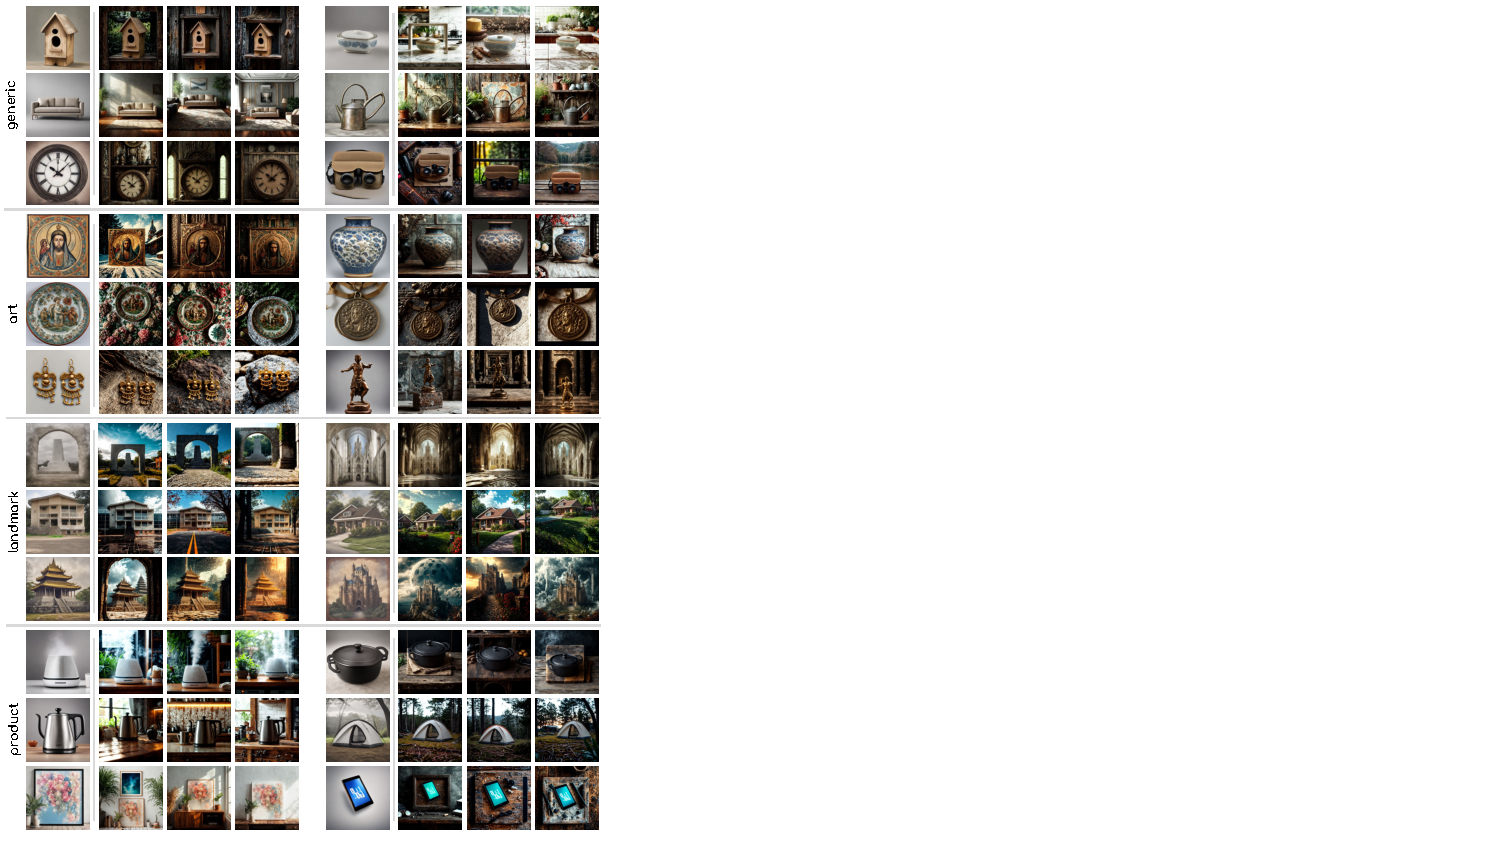
\includegraphics[width=0.91\linewidth]{fig/example.pdf}
\vspace{-9pt}
\caption{Examples of object instances generated by GDM (column 1), and the generated images that leave the object intact and add lighting and background that is well suited to the object (columns 2 $\sim$ 4).
\label{fig:iclight}}
\end{figure*}

\subsection{Representation learning}
%
In total, our generated dataset contains $CKN$ training images, forming $CK$ classes coming from $C$ object categories. 
We construct training batches by sampling $B$ classes and all their corresponding images, resulting in $NB$  images per batch. 
During training, we adopt a query \vs database scheme:
one image from each of the $N$ images per class is randomly chosen as the query, while the remaining $NB-1$ images of the batch form the database, as shown in \cref{fig:batch}.

The similarity between the query and db images is computed in $\hat{\mathbf{y}} \in \mathbb{R}^{NB-1}$, while $\mathbf{y} \in \{0,1\}^{NB-1}$ denotes the labels of all db images with respect to the query, \ie positive or negatives based on their classes. 
We optimize an information retrieval metric as the loss function, in particular an approximation of recall at the top-$k$ ranks, based on $\hat{\mathbf{y}}$, and $\mathbf{y}$.
We train with the average of recall@k loss estimated for different values of $k$.
The approximation of recall is possible by formulating its estimation with the use of step functions, which, during training, are replaced with a sigmoid function.
The technical and implementation details can be found in the original paper~\citep{ptm22}.





\begin{figure}[t]
\begin{center}
\includegraphics[width=0.83\linewidth]{fig/batch.pdf}
\vspace{-10pt}
\caption{Training batch construction for instance-level representation learning. A batch simulates a retrieval task with a query (blue) and database of positive (green) and negative (red) images. Images are considered positive if they belong to the same class, otherwise they are negatives. An image encoder is trained with metric learning on this batch.}
\label{fig:batch}
\end{center}
\end{figure}

\begin{table}[t]
    \centering
    \caption{Statistics of the generated training dataset. \oursgeneric{} and \oursspecific{} comprise only objects from the generic domain and one of the specific domains, respectively.  
    \oursplus{} comprises 50\% of objects from the generic domain ($10$K) and all objects from the three specific domains ($10$K), \ie $20$K objects in total.}
\small
\begin{tabular}{lrrr}
\toprule
\textbf{domain of objects}  & $C$ & $K$ & \textbf{instances} \\ 
\midrule
generic           & $2,000$  & $10$ & $20,000$ \\ 
art        & $200$  & $15$ & $3,000$ \\ 
landmark   & $50$ & $80$  & $4,000$ \\
product    & $200$ & $15$  & $3,000$ \\  
\bottomrule
\end{tabular}

\label{tab:gene_details}
\end{table}


\section{Experiments}
\label{sec:exp}

\subsection{Implementation Details}
\label{sec:impl}

We select Wan2.1~\citep{wan} as the base I2V model to apply IF-V2V. It can generate 480p videos with 14B parameters. We adopt the Euler Discrete Scheduler~\citep{sd3} to solve the ODE with $t_{max}=0.95$ and 25 sampling steps. Classifier-free guidance with scale $5.0$ is applied when predicting the target denoising vector. The rectification scale $\lambda$ in \sref{sec:vfr-sd} is set to $1.0$. The embedding scale $\beta$ and the blending factor $\alpha$ in \sref{sec:smpi} are selected as $0.025$ and $0.95$, respectively. The caching threshold $\delta$ in \sref{sec:dcache} is set to $0.5$. All other hyperparameters remain the same as Wan2.1~\citep{wan}. Experiments are conducted on NVIDIA RTX 4090 GPUs.

\subsection{Qualitative Results}
\label{sec:qualitative}

\begin{figure}
  \centering
  \includegraphics[width=\linewidth]{figs/vis.pdf}
  % \vspace{-20pt}
  \caption{Editing results of IF-V2V (\sref{sec:qualitative}). In each case, the first row presents the original video, and the other rows show the edited video with the first frame condition in the bottom-right corner. 
  % The cases include attribute modification (a, c, e.1, and f.1), text insertion (b), object removal (d), and stylization (e.2 and f.2). Our method propagates the edited frame through the temporal dimension with satisfactory quality and consistency.
  % \anyi{add more captions}
  }
  \label{fig:vis}
\end{figure}

We present various creative video editing results using IF-V2V in \cref{fig:teaser,fig:vis}, including attribute modification (teaser, a, c.1, and d.1), object addition (teaser), object removal (b), and stylization (c.2 and d.2). As observed, IF-V2V achieves satisfying visual quality and consistency on a wide variety of image-conditioned video editing tasks thanks to the graceful collaboration between state-of-the-art image editing approaches~\citep{gpt4oimg, stepedit} and I2V models~\citep{wan} empowered by our method. More results can be found in \sref{sec:vis_extra} and the supplementary video.

\subsection{Comparisons to Prior Works}
\label{sec:comparison}

\subsubsection{Quantitative Comparisons}
\label{sec:comparison_quantitative}

To further demonstrate the superiority of IF-V2V over other methods, we quantitatively evaluate these approaches on 40 editing samples from the DAVIS~\citep{davis} dataset and in-the-wild videos with a maximum of 81 frames. We construct these samples by editing the first frame of the video with GPT-4o~\citep{gpt4oimg} and Step1X-Edit~\citep{stepedit}. We employ the following metrics to assess the editing quality: 1) \textit{Aesthetics Score (AS)}~\citep{laion5b}: this metric evaluates the per-frame visual quality of the generated video. 2) \textit{Temporal Consistency (TC)}: it assesses the smoothness of the edited video by calculating the average cosine similarity of CLIP~\citep{clip} visual embeddings between every 2 consecutive frames. 3) \textit{Edited Frame Consistency (EFC)}: it represents the consistency between the edited first frame and the generated video by the average cosine similarity of CLIP~\citep{clip} visual embeddings. 4) \textit{Human Preferences (HP)}: it stands for 13 volunteers' average rating on editing quality (5-point Likert Scale).

\begin{table}
  \centering
  \caption{Quantitative results. \textbf{Bold} results are the best and \underline{underlined} results are the second best.}
  \begin{subtable}{0.435\linewidth}
      \caption{Comparisons with prior arts (\sref{sec:comparison_quantitative}). 
      % Results in \textbf{bold} are the best.
      \dag~Reference-based V2V without mask input.
      % \anyi{Do we need to stress up this is training-based and our is training-free?}
      }
      \label{tab:quantitative}
      \centering
      \resizebox{1\linewidth}{!}{
      \begin{tabular}{l|ccc|c}
        \toprule
        Method & AS & TC & EFC & HP \\
        \midrule
        Videoshop & 4.62 & 97.87 & 76.85 & 1.69 \\
        AnyV2V & \underline{4.81} & 97.88 & \underline{81.47} & \underline{2.56} \\
        VACE\textsuperscript{\dag} & 4.57 & \underline{97.94} & 75.65 & 1.64 \\
        IF-V2V (Ours) & \textbf{4.88} & \textbf{98.71} & \textbf{92.79} & \textbf{4.50} \\
        \bottomrule
      \end{tabular}}
  \end{subtable}
  \hfill
  \begin{subtable}{0.555\linewidth}
      \caption{Component ablations of IF-V2V (\sref{sec:diagnostic_quantitative}).}
      \label{tab:ablation}
      \centering
      \resizebox{1\linewidth}{!}{
      \begin{tabular}{l|ccccc|c}
        \toprule
        Setting & AS & TC & EFC & OVC & AEC & Time \\
        \midrule
        I2V & 4.88 & 98.70 & 93.71 & 75.03 & 84.37 & 554.27 \\
        I2V + Init & 4.89 & 98.30 & 88.34 & 78.74 & 83.54 & 553.52 \\
        \midrule
        \textit{w/o} VFR-SD & 4.87 & 98.29 & 91.23 & 75.27 & 83.25 & \textbf{553.58} \\
        \textit{w/o} SMPI & 4.78 & 98.19 & 92.67 & 75.45 & 84.06 & 622.38 \\
        \textit{w/o} D-Cache & \underline{4.87} & \underline{98.41} & \textbf{93.37} & \textbf{76.61} & \textbf{84.99} & 804.46 \\
        IF-V2V & \textbf{4.88} & \textbf{98.71} & \underline{92.79} & \underline{76.44} & \underline{84.62} & \underline{616.60} \\
        \bottomrule
      \end{tabular}}
    \end{subtable}
\end{table}

% TODO: add flowedit

We compare IF-V2V with inversion-based methods, Videoshop~\citep{videoshop} and AnyV2V~\citep{kuanyv2v}, and a training-based method, VACE~\citep{vace}. For VACE, we compose the inputs as a reference-based V2V task without the mask input. As displayed in \cref{tab:quantitative}, IF-V2V consistently outperforms other approaches across all metrics, especially on EFC and HP. Compared to the inversion-based prior art AnyV2V~\citep{kuanyv2v}, our method achieves consistently better results without inversion and model-specific design. Training-based method VACE~\citep{vace} also falls behind our method when no editing mask is provided.

\begin{figure}
  \centering
  \includegraphics[width=\linewidth]{figs/vis_comp.pdf}
  % \vspace{-20pt}
  \caption{Qualitative comparisons with previous methods (\sref{sec:comparison_qualitative}). The edited first frame is in the bottom-right corner of the source video.}
  \label{fig:comparison_qualitative}
\end{figure}

\subsubsection{Qualitative Comparisons}
\label{sec:comparison_qualitative}
We visualize the edited videos in \cref{fig:comparison_qualitative} to provide an intuitive comparison with other methods. The left side shows an object addition task, where Videoshop and VACE exhibit significant artifacts. Although AnyV2V adds the blue scarf and preserves the dog's motion, the hue gets less vivid, and the background becomes blurry. Our method achieves the best result in inserting the blue scarf while maintaining the other aspects of the video. On the right side, we expect the models to alter the input video's style according to the given first frame. All the methods fail in this task except IF-V2V, further validating its effectiveness.

\subsection{Diagnostic Experiments}
\label{sec:diagnostic}

\subsubsection{Quantitative Ablations}
\label{sec:diagnostic_quantitative}

To provide a better understanding of IF-V2V's components, we conduct ablation studies on the same editing samples as \sref{sec:comparison_quantitative}. Besides the objective metrics in \sref{sec:comparison_quantitative}, we additionally adopt the following metrics: 1) \textit{Original Video Consistency (OVC)}: this metric measures the per-frame consistency between the edited video and the original video by the average cosine similarity of CLIP~\citep{clip} visual embeddings. 2) \textit{Average Editing Consistency (AEC)}: it is the mean value of EFC and OVC to assess the general editing consistency. 3) \textit{Time}: it is the average time taken per video for the editing process in seconds.

We present the quantitative results in \cref{tab:ablation}. Two baseline methods are compared in the first two rows. I2V (\#1) represents the result for directly adopting an I2V model~\citep{wan}. Although it achieves high TC and EFC, a large portion of the generated videos are \textit{almost still}, which accounts for the high consistency scores. The OVC of \#1 is also low because there is no information from the source video during generation. I2V + Init (\#2) stands for using the I2V model~\citep{wan} with initial latents generated by the linear combination of Gaussian noise and source video latents. Despite enhanced OVC, EFC significantly drops because information from the source video becomes dominant, and the model fails to integrate information from the edited frame.

\#3 demonstrates the results without VFR-SD. Despite the fastest inference time, EFC, OVC, and AEC are significantly behind those of IF-V2V (\#6), demonstrating the capability of VFR-SD to incorporate characteristics of the source video while temporally propagating the edited frame.

\#4 shows the metrics without SMPI. Compared to IF-V2V (\#6), the drop of AS, TC, and OVC is relatively prominent. This validates SMPI's effect on better preserving the details in the original video to enhance the visual quality of the editing result.

\#5 presents the results without the D-Cache mechanism. Despite slightly improved EFC, OVC, and AEC, the inference time increases significantly (\textbf{+30.5\%}) compared to IF-V2V (\#6), attesting to the acceleration effectiveness of D-Cache without notably compromising editing quality.

\begin{figure}
  \centering
  \includegraphics[width=\linewidth]{figs/vis_abl.pdf}
  \caption{Case study for components (\sref{sec:diagnostic_case_study}).
  % for IF-V2V's components 
   % The source video shows a grey van driving up a hill along the road. 
  We edit the first frame to be a white car with its \textbf{back towards the uphill direction}, expecting to generate a creative video in which the white car drives \textbf{backwards} up the hill. The edited first frame is in the bottom-right corner of the source video.}
  \label{fig:case_study}
\end{figure}

\subsubsection{Case Study}
\label{sec:diagnostic_case_study}

We further demonstrate the functions of IF-V2V's components with a creative editing sample in \cref{fig:case_study}, which originally shows a grey van driving upwards a hill along the road. We edit the first frame to be a \textbf{white car} with its \textit{back towards the uphill direction}, with an expectation of generating a creative video in which the white car drives \textit{backwards} along the road up the hill.

If we directly generate the video with the I2V model~\citep{wan} (\#2), it fails to follow the text prompt, resulting in the white car driving forward down the hill. Initializing the latents with the source video as \sref{sec:diagnostic_quantitative} (\#3) does let the white car drives up the hill, but the generated car has obvious artifacts with \textit{both sides being the back}. Meanwhile, this approach also suffers from inconsistent road shape and blurry output videos.

Results in \#4 illustrates that without VFR-SD, the synthesized car also has two back ends. Meanwhile, there is a little corruption at the end of the road. The comparison between \#4 and \#6 displays that VFR-SD better preserves information from the source video, resulting in a more consistent and reasonable output. In \#5, the white car first moves backwards for a little distance, then drifts towards the front right. Without SMPI, the method fails to preserve the motion from the source video.

Both \#6 and \#7 successfully propagate the edited first frame to the source video to generate a white car driving backwards up the hill. We can observe that IF-V2V with D-Cache mechanism offers an effective and user-friendly solution for creative editing with reasonable overhead.

% leveraging the combination of any black-box image editing models and flow-based I2V models.



\section {Conclusion}
\vspace{-3mm}
% 不同于现有方法在“层”维度对特征做缓存优化,FreqCa 首次将加速视角转向“频域”,它将累积残差特征按频域分解为低频与高频分量,二者遵循截然不同的时序演化规律,并据此采用针对性策略低频保结构、高频精预测,既规避了跨层误差传播,又契合扩散过程的时序平滑性。FreqCa 揭示了从频域、结构与时序三个维度协同理解和建模特征的变化

% 实验表明,这一设计不仅在 FLUX、Qwen-image 等主流生成模型上实现 >90% 显存压缩与 普遍6-7倍的几乎无损加速,更在图像编辑等下游任务中展现出卓越泛化能力。未来,针对模型输出的频域建模预测为资源受限场景下的高效生成提供通用范式。
In this work, we presented \textbf{\textit{FreqCa}}, a frequency-aware feature caching framework that unifies the strengths of reuse- and forecast-based paradigms. By decomposing features into low- and high-frequency components, \textit{FreqCa} selectively reuses stable low-frequency features and accurately predicts dynamic high-frequency components, leading to a superior trade-off between acceleration and generation quality. Furthermore, by introducing Cumulative Residual Feature caching, we reduced the memory footprint to $\mathcal{O}(1)$, making frequency-aware caching practical even on consumer hardware. Extensive experiments across diverse diffusion models demonstrate that \textit{FreqCa} achieves 6–7$\times$ acceleration with negligible quality degradation, establishing a new SOTA in efficient diffusion inference. We believe \textit{FreqCa} opens up new possibilities for scalable, high-performance generative modeling and offers a general method for future research in frequency-aware acceleration techniques.

% \subsubsection*{Author Contributions}
% If you'd like to, you may include  a section for author contributions as is done
% in many journals. This is optional and at the discretion of the authors.

% \subsubsection*{Acknowledgments}
% Use unnumbered third level headings for the acknowledgments. All
% acknowledgments, including those to funding agencies, go at the end of the paper.


\bibliography{iclr2026_conference}
\bibliographystyle{iclr2026_conference}

\appendix
\section*{Appendix Overview}

The appendix includes extra experimental results, corresponding analyses, and further discussions of IF-V2V. The appendix is organized as follows:
\begin{itemize}
    \item \sref{sec:diagnostic_lambda} analyzes the effect of the rectification scale in \sref{sec:vfr-sd}.
    \item \sref{sec:abl_smpi} further ablates the components of SMPI.
    \item \sref{sec:comp_solver} provides comparisons on adopting different ODE solvers.
    \item \sref{sec:ext_flow} demonstrates quantitative and qualitative results of extending IF-V2V to other flow-based I2V models for editing.
    \item \sref{sec:t2v_edit} presents qualitative results of extending IF-V2V for text-guided video editing.
    \item \sref{sec:image_edit} adapts an inversion-free image editing method FlowEdit~\citep{kulikov2024floweditinversionfreetextbasedediting} to the video domain for quantitative comparison.
    \item \sref{sec:vis_extra} shows more qualitative results of IF-V2V.
    \item \sref{sec:discussions} further discusses the theoretical justifications, hyperparameter selection criteria, limitations, and societal impacts of IF-V2V.
\end{itemize}

\section{Effect of the Rectification Scale}
\label{sec:diagnostic_lambda}

\begin{figure}[ht]
  \centering
  \includegraphics[width=\linewidth]{figs/vis_lambda.pdf}
  \caption{Illustration of the effect of the rectification scale $\lambda$ (\sref{sec:diagnostic_lambda}). The source video shows a boy in a \textbf{white} T-shirt cycling along the road, and the edited first frame changes the boy's T-shirt to \textbf{red}. The value of $\lambda$ can be tuned in an appropriate range to control the strength of the source video prior. A small $\lambda$ ($\leq 0.50$) brings a weak prior from the source video, resulting in inconsistency with the source video that the boy cycles along a road with an endless wall. When $\lambda$ is too large ($\geq 1.25$), artifacts like blurs and oversaturation also emerge. Please zoom in for details.}
  \label{fig:lambda}
\end{figure}

The rectification scale $\lambda$ in \sref{sec:vfr-sd} determines the strength that VFR-SD incorporates the source video's deviation from expectation during the target ODE solving process. To provide an intuitive understanding of the impact of $\lambda$ on the edited video, we present a visualization of using different values of $\lambda$ to edit a video sample in \cref{fig:lambda}. The video originally captures a boy in a white T-shirt cycling along the road, and the edited frame turns the boy's T-shirt red. When $\lambda$ is small ($\leq 0.5$), the deviation from the source video is relatively weak, and the denoising process resembles the straightforward I2V process. In this case, the sample deviation is inadequate to direct the denoising process, resulting in the boy cycling along the road with an \textit{endless} wall. In contrast, an overly large $\lambda$ value ($\geq 1.25$) also induces artifacts like blurs and oversaturation because the rectification term pushes the generated sample too far from the original distribution.

\section{Extra Ablations on SMPI}
\label{sec:abl_smpi}

We conduct extra ablations to provide a better understanding of SMPI. The results are displayed in \cref{tab:abl_smpi}, where \textit{w/o} MPI stands for without motion-preserving initialization. Comparing \#1 and \#2, we can observe that structure-preserving initialization better maintains the consistency with original videos (OVC). From \#2 and \#3, it can be concluded that motion-preserving initialization further enhances temporal consistency.

\begin{table}[ht]
  \caption{Quantitative ablations on SMPI (\sref{sec:abl_smpi}). Results in \textbf{bold} are the best.
  }
  \label{tab:abl_smpi}
  \centering
  \begin{tabular}{l|ccccc|c}
    \toprule
    Setting & AS & TC & EFC & OVC & AEC & Time \\
    \midrule
    \textit{w/o} SMPI & 4.78 & 98.19 & 92.67 & 75.45 & 84.06 & 622.38 \\
    \textit{w/o} MPI & 4.81 & 98.06 & 92.51 & 76.30 & 84.41 & \textbf{615.17} \\
    IF-V2V & \textbf{4.88} & \textbf{98.71} & \textbf{92.79} & \textbf{76.44} & \textbf{84.62} & 616.60 \\
    \bottomrule
  \end{tabular}
\end{table}

\section{Comparisons on ODE Solvers}
\label{sec:comp_solver}

To validate IF-V2V's compatibility with different ODE solvers, we evaluate IF-V2V's performance with Euler Discrete Scheduler~\citep{sd3} and UniPC Scheduler~\citep{unipc}. Quantitative results are displayed in \cref{tab:comp_solver} with the same settings as \sref{sec:diagnostic}. We also present qualitative results in \cref{fig:vis_solver}. From the above results, we can conclude that IF-V2V also achieves satisfactory performance with UniPC Scheduler~\citep{unipc}, demonstrating the universality of our method.

\begin{table}
  \caption{Comparisons on adopting different ODE solvers in IF-V2V (\sref{sec:comp_solver}).
  % Results in \textbf{bold} are the best.
  }
  \label{tab:comp_solver}
  \centering
  \begin{tabular}{l|ccccc}
    \toprule
    Setting & AS & TC & EFC & OVC & AEC \\
    \midrule
    UniPC~\citep{unipc} & 4.86 & 98.70 & 92.01 & 76.48 & 84.25  \\
    Euler~\citep{sd3} & 4.88 & 98.71 & 92.79 & 76.44 & 84.62 \\
    \bottomrule
  \end{tabular}
\end{table}

\begin{figure}[ht]
  \centering
  \includegraphics[width=\linewidth]{figs_supp/vis_solver.pdf}
  \caption{Visualizations of using different ODE solvers in IF-V2V (\sref{sec:comp_solver}). The edited first frame is in the bottom-right corner of the edited video. IF-V2V is compatible with multiple ODE solvers to produce high-quality editing results.}
  \label{fig:vis_solver}
\end{figure}

\section{Extension to Other Flow-based I2V Models}
\label{sec:ext_flow}

\begin{table}
  \caption{Comparisons on using different I2V models in IF-V2V (\sref{sec:ext_flow}).
  % Results in \textbf{bold} are the best.
  }
  \label{tab:comp_flow}
  \centering
  \begin{tabular}{l|ccccc}
    \toprule
    Setting & AS & TC & EFC & OVC & AEC \\
    \midrule
    % \makecell[l]{HunyuanVideo\\\citep{hunyuanvideo}} & 4.75 & 98.60 & 92.92 & 75.36 & 84.14  \\
    HunyuanVideo~\citep{hunyuanvideo} & 4.75 & 98.60 & 92.92 & 75.36 & 84.14  \\
    Wan2.1~\citep{wan} & 4.88 & 98.71 & 92.79 & 76.44 & 84.62 \\
    \bottomrule
  \end{tabular}
\end{table}

\begin{figure}
  \centering
  \includegraphics[width=\linewidth]{figs_supp/vis_hunyuan.pdf}
  \caption{Editing samples of using different flow-based I2V models in IF-V2V (\sref{sec:ext_flow}). The edited first frame is in the bottom-right corner of the source video. IF-V2V can be applied to various flow-based I2V models for high-quality video editing.}
  \label{fig:vis_hunyuan}
\end{figure}

To further demonstrate the universality of IF-V2V, we select HunyuanVideo~\citep{hunyuanvideo} as another base I2V model to apply our method. We present the quantitative results in \cref{tab:comp_flow}, from which we can find that HunyuanVideo~\citep{hunyuanvideo} also achieves a satisfying result that surpasses prior arts. \cref{fig:vis_hunyuan} shows the visualization of some editing cases, in which we can observe that both HunyuanVideo~\citep{hunyuanvideo} and Wan2.1~\citep{wan} achieve excellent consistency with both the edited frame and the original video with the help of IF-V2V.

\section{Extension to Text-guided Editing}
\label{sec:t2v_edit}

\begin{figure}
  \centering
  \includegraphics[width=\linewidth]{figs_supp/vis_t2v.pdf}
  \caption{Text-guided editing results of IF-V2V (\sref{sec:t2v_edit}). We provide the simplified editing caption under each sample. Compared to \textit{I2V + Init}, our method preserves the details more faithfully, like shells and splashes in (a), and aligns better with the editing instruction, such as the guitar in (b).}
  \label{fig:vis_t2v}
\end{figure}

IF-V2V can also be used for text-guided video editing by removing the condition embedding in Structure-Preserving Initialization. We present some qualitative results using Wan2.1~\citep{wan} as the text-to-video model in \cref{fig:vis_t2v}, in which we can observe that IF-V2V also achieves excellent consistency and editing quality. In \cref{fig:vis_t2v} (a), IF-V2V keeps the details more faithfully, such as shells on the beach and splashes in the sea, compared to directly blending Gaussian noise and source video latents as the initial condition for the I2V model (I2V + Init). In \cref{fig:vis_t2v} (b), IF-V2V also aligns better with the editing prompt that alters the electric guitar into a normal one.

\section{Quantitative Comparisons with FlowEdit}
\label{sec:image_edit}

To demonstrate the superiority of IF-V2V over directly adopting image-based inversion-free editing methods for videos, we adapt FlowEdit~\citep{kulikov2024floweditinversionfreetextbasedediting}, a flow-based inversion-free image editing method, for video editing on Wan2.1~\citep{wan}. The performance is displayed in \cref{tab:comp_flowedit}, from which we can observe that both its editing quality and inference speed remain inferior to IF-V2V. This further validates the effectiveness of our new perspective on the ODE solving process, video-specific designs, and flexible caching strategy.

\begin{table}
  \caption{Quantitative comparisons with FlowEdit (\sref{sec:image_edit}). Results in \textbf{bold} are the best.}
  \label{tab:comp_flowedit}
  \centering
  \begin{tabular}{l|ccc|c}
    \toprule
    Setting & AS & TC & EFC & Time \\
    \midrule
    FlowEdit~\citep{kulikov2024floweditinversionfreetextbasedediting} & 4.76 & 98.01 & 92.32 & 802.42 \\
    IF-V2V (Ours) & \textbf{4.88} & \textbf{98.71} & \textbf{92.79} & \textbf{616.60}\\
    \bottomrule
  \end{tabular}
\end{table}

\section{More Visualizations}
\label{sec:vis_extra}

We illustrate more editing results of IF-V2V in \cref{fig:vis_extra}, which include object addition (a), object removal (b), and attribute modification (c). As observed, IF-V2V consistently achieves satisfactory performance on various video editing tasks. Please refer to the supplementary video for dynamic versions of editing samples.

\begin{figure}
  \centering
  \includegraphics[width=\linewidth]{figs/vis_extra.pdf}
  \caption{More visualizations of editing results of IF-V2V (\sref{sec:vis_extra}). The edited first frame is in the bottom-right corner of the source video. The cases include object addition (a), object removal (b), and attribute modification (c). Our method propagates the edited frame to the whole video with excellent quality and consistency.
  }
  \label{fig:vis_extra}
\end{figure}

\section{More Discussions}
\label{sec:discussions}

\subsection{Theoretical Justifications}
\label{sec:theoretical}
IF-V2V shares a similar theoretical basis as inversion-based editing methods: Optimal Transport (OT) mapping between the source and target distribution. The theoretical difference is that inversion-based methods conduct a mapping on the marginal distribution $p(z_0|z_{t_{max}})$, while IF-V2V performs mappings on transition distributions $p(z_{t-\Delta t} |z_t)$. When \(\Delta t\) is small enough, both the source and target transition distributions can be viewed as Gaussians with the same variance~\citep{ddpm, gmflow}. In this case, IF-V2V with $\lambda=1$ performs the exact OT mapping on the transitions.

\subsection{Hyperparameter Selection}
\label{sec:hyperparam}

The editing results suffer from over-saturation and distortion when the rectification scale $\lambda$ in \sref{sec:vfr-sd} is overly large. When the edited frame is not aligned with the original frame, the rectification sometimes causes unintended drifts due to the conflict. The scale of structure-preserving initialization $\beta$ in \sref{sec:spi} should be small enough when the edited region is large. Otherwise, IF-V2V mostly preserves the original video. An overly large flow-guided initialization factor $\alpha$ in \sref{sec:mpi} breaks the temporal Gaussianity of the noise and fails the generation.

It has been discovered that initial steps are more crucial for editing, and the vector difference in these steps is also larger. The caching threshold $\delta$ in \sref{sec:dcache} is selected around the vector difference in early steps to avoid caching these steps. Caching in later steps reduces computational cost with less impact on editing quality.

\subsection{Limitations}
\label{sec:limitations}

The editing capability of our method is inherently bounded by the selected image editing model and the I2V model. Failure in either stage will result in unsatisfactory results. Moreover, since existing I2V models only predict the expectation of the distribution without covariance information, IF-V2V cannot exploit the covariance to achieve more precise mapping from the source sample to the target sample in a training-free way. 

\subsubsection{Image Editing Methods}
\label{sec:limitations_imageedit}

IF-V2V's editing results rely on the first frame edited by image editing methods. However, current state-of-the-art methods~\citep{gpt4oimg, stepedit} still suffer from inconsistencies and trial-and-error. For instance, the image edited by GPT-4o~\citep{gpt4oimg} often misaligns with the original image, especially when changing the original image into a significantly different style (\eg, Ghibli cartoonish style). Such misalignment may cause undesired alterations in the edited videos. In addition, Step1X-Edit~\citep{stepedit} sometimes needs several tries to achieve a satisfactory editing result. We expect that the future advancements of image editing methods will ease the process of obtaining a satisfactory first frame and further boost the performance of IF-V2V.

\subsubsection{I2V Models}
\label{sec:limitations_i2v}

\begin{figure}
  \centering
  \includegraphics[width=\linewidth]{figs_supp/vis_failure.pdf}
  \caption{Failure cases of IF-V2V (\sref{sec:limitations_i2v}). The edited first frame is in the bottom-right corner of the source video. IF-V2V struggles to handle editing samples with overly complex (a) or fast (b) motions due to the limited capability of I2V models.}
  \label{fig:failure}
\end{figure}

IF-V2V fails to produce satisfactory results when motion in the source video is overly complex or fast. As \cref{fig:failure} (a) displays, when there are complicated motions in the source video like simultaneous multiple subject movement with changing occlusions, IF-V2V cannot genuinely reproduce such motion in the edited video. In \cref{fig:failure} (b), IF-V2V generates unsatisfactory results when dealing with breakdance, which contains rapid human body movements. These phenomena stem from state-of-the-art I2V models' limited ability to generate rapid or sophisticated motions. This problem may be resolved by more powerful I2V models in the future which are capable of handling such complex motions.

Furthermore, mainstream flow-based I2V models~\citep{wan, easyanimate, hunyuanvideo, cogvideox, opensora2, vchitect2} only predict the \textit{expectation} of the target distribution without further information like covariance, making it hard to conduct more fine-grained operations to map the source sample to the target distribution in a training-free way. This may limit the method's ability to maintain the consistency of fine-grained details in edited videos.

\subsection{Societal Impacts}
\label{sec:impacts}

IF-V2V can achieve high-quality video editing by combining off-the-shelf image editing and I2V methods without training, enabling practitioners to flexibly leverage the most up-to-date models to implement their creativity. For individual creators, the lightweight nature of our method enables them to introduce AI-assisted video content creation into their workflow, democratizing the application of advanced AIGC tools. This shift can also expand storytelling beyond traditional media institutions to include diverse voices and perspectives. For commercial teams, our method provides them with a new chance to flexibly combine their internal results or models with the progress of the open-source community, boosting the quality of the produced videos with minor extra cost.

On the other hand, with IF-V2V's powerful capability of manipulating objects and attributes in the video, it can produce fabricated videos that appear highly realistic, posing significant challenges for verifying the authenticity of visual media. Such content can distort public perception and raise privacy concerns when fake contents featuring an individual are generated in an unauthorized way.


\end{document}
